\documentclass[12pt,a4paper]{article}

\usepackage{anyfontsize}
\usepackage{graphicx}

%package for list formatting (ordered) if we add [a.]
\usepackage{enumerate}
%package for graphics or include images
\usepackage{graphicx}
\usepackage{float} %to place image forcefully there

\usepackage{subcaption,caption}
\usepackage[hidelinks]{hyperref}

%for times new roman font
\usepackage{times,mathptmx}


%package for margins
\usepackage[outer=1.25in,inner=1.5in,top=1in,bottom=1in,headheight=0.5in,footskip=0.5in]{geometry}
%better to use outer and inner beacause while printing book then right and left margin will not be good , So, inner margin 


\begin{document}
	\pagenumbering{roman}
	
	
\begin{titlepage}
	
	\newcommand{\HRule}{\rule{\linewidth}{0.3mm}}
	\centering
	\vfill
	
\includegraphics[width=50mm]{images/tu.jpg}\\[0.75cm]
	\textsc{\Large \bfseries  TRIBHUVAN UNIVERSITY}\\[0.25cm] % Name of your university/college
	\textsc{\Large \bfseries INSTITUTE OF ENGINEERING}\\[0.25cm]
	\textsc{\Large \bfseries  PULCHOWK CAMPUS}\\
	\vfill
	\large {A PROJECT REPORT ON }\\
	\Large \textbf{Tetris: The Classic Puzzle Game}
	\vfill
	%\large \textbf{Subject code} \\[0.2cm]
%	\bfseries
	\large
		\textbf{Submitted by:}\\
	AASHISH KARKI (078BCT004)\\
	ANUP ARYAL (078BCT015)\\
	APIL CHAUDHARY (078BCT017)\\[0.5cm]
	\vfill
		\textbf{SUBMITTED TO:}\\
	DEPARTMENT OF ELECTRONICS AND COMPUTER ENGINEERING\\
	IOE, Pulchowk Campus\\
	Kathmandu Nepal
	\\
	\vfill
	{\large \today}
	\vfill
\end{titlepage}

	
  	
  	
  	\newpage
\pagenumbering{arabic}
\section{ACKNOWLEDGEMENT}


We express our sincere gratitude to our teachers(Mr. Daya Sagar Baral, Mr. Aman Shakya and Mr. Rajad Shakya) who suggested building this game for sharpening our Object Oriented Programming skills and logic building capabilities.

\vspace{5mm}
Our special thanks goes to our lecturer, Daya Sagar Baral, for his guidelines, suggestions, and instructions, which have served as a contributor towards the inception of this project.

\vspace{5mm}
We sincerely thank the Department of Electronics and Computer Engineering, Pulchowk Campus, for giving us an opportunity to work on this project to expand our knowledge of Object Oriented Programming and working in a team.

  	\input{sec/Abstract}
  	
  	\newpage
  	{
  		\setlength{\parskip}{0em}
  	%	\renewcommand\contentsname{TABLE OF CONTENTS}\\[0.5cm] % This will change heading text
  		\tableofcontents 
  	   % \addcontentsline{toc}{section}{TABLE OF CONTENTS}
  	}
  	
  	
  	\newpage
\section{OBJECTIVES}
The objectives of building this game in C++ are listed below:


\begin{enumerate}
\item \textbf{Use Object-Oriented Programming (OOP):}
	\begin{itemize}
		\item Create classes for Tetrominoes, game board, and game logic.
		\item Organize code for easy maintenance and flexibility.
	\end{itemize}
	
\item \textbf{Explore C++ Features:}
\begin{itemize}
	\item Manage game data efficiently using vectors, pairs, maps and other containers in STL.
	\item Handle resources smartly to optimize performance.
\end{itemize}

\item \textbf{Graphics with SFML:}
\begin{itemize}
	\item Use SFML to draw Tetrominoes, game board, and animations.
	\item Respond to player input using SFML's event system.
\end{itemize}

\item \textbf{Reusable Code:}
\begin{itemize}
	\item Create header files for sharing code across the game.
\end{itemize}

\item \textbf{Implement Game Mechanics:}
\begin{itemize}
	\item Make Tetrominoes rotate, move, and detect collisions.
	\item Create a scoring system and difficulty levels.Create a scoring system and difficulty levels.Create a scoring system and difficulty levels.
\end{itemize}

\item \textbf{Add Sound Effects and Music:}
\begin{itemize}
	\item Integrate audio using SFML for a better gaming experience.
\end{itemize}

\item \textbf{Test and Debug:}
\begin{itemize}
	\item Thoroughly test the game to fix any issues.
	\item Use logs and debugging tools for troubleshooting.
\end{itemize}

\item \textbf{Team Collaboration:}
\begin{itemize}
	\item Communicate well within the team.
	\item Use Git for version control and collaboration.
\end{itemize}
\end{enumerate}
  	\newpage
\pagenumbering{arabic}
\section{INTRODUCTION}
\hspace{5mm}Tetris, an iconic and enduring puzzle game, has captured the hearts of gamers around the world since its inception in 1984. Created by Russian game designer Alexey Pajitnov, Tetris challenges players with a deceptively simple objective: fitting different-shaped blocks, known as tetrominoes, together to form complete lines. Yet, beneath its straightforward premise lies an addictive and exhilarating experience that has stood the test of time.\\

\textbf{Gameplay :} \\

\textbf{Tetrominoes:} The game consists of various tetrominoes, each made up of four connected squares arranged in different shapes. The seven tetrominoes are: I, J, L, O, S, T, and Z.\\

\textbf{Falling Blocks: }Tetrominoes fall from the top of the playing area one at a time. You have the ability to move and rotate the tetrominoes as they descend.\\

\textbf{Movement and Rotation:} You can move the falling tetrominoes horizontally (left or right) using the arrow keys or buttons. You can also rotate them clockwise or counterclockwise to fit them into available spaces using the up arrow key or designated rotation buttons.\\

\textbf{Clearing Lines:} The primary goal is to create complete horizontal lines by filling all the spaces within a row. When a line is entirely filled, it clears from the screen, and you earn points.\\

\textbf{Scoring:} The more lines you clear at once, the higher the points you earn. Clearing multiple lines simultaneously is known as a "Tetris" and yields the highest points.\\

\textbf{Leveling Up:} As you accumulate points or clear a certain number of lines, you advance to higher levels. With each level, the tetrominoes fall faster, increasing the game's difficulty.\\

\textbf{Game Over:} The game ends when the stack of falling tetrominoes reaches the top of the playing area. If you can't clear lines fast enough, the stack will reach the top, and the game will be over.\\

\textbf{Controls:}\vspace{5mm}\\
The controls for Tetris are usually straightforward:\\
\textbf{Left Arrow: }Move tetromino left\\
\textbf{Right Arrow: }Move tetromino right\\
\textbf{Down Arrow: }Accelerate the fall of the tetromino\\
\textbf{Up Arrow: }Rotate tetromino clockwise or counterclockwise\\


  	\newpage
\section{APPLICATIONS}


		\hspace{5mm}Tetris was originally inspired by a puzzle game called "pentominoes," in which different wooden shapes made of five equal squares are assembled in a box. Hence, Tetris is also a puzzle in itself and thus a “mind” game. Although, video games are often dismissed as unsophisticated or the domain of couch potatoes, but many common elements of these simulated worlds can provide tangible benefits in real life. Benefits of Tetris for both children and adults include:
		\begin{itemize}
			\item Healthy Brain Simulation
			\item Development of Problem Solving Skills
			\item Stress Relief
		\end{itemize}
		
		\hspace{5mm}Taking these benefits into account, application of Tetris are discussed below:
		
			\begin{enumerate}
				\item \textbf{Problem Solving:} As already mentioned above, Tetris is a puzzle game and thus, is a tool to develop problem solving skills. Placing each block requires a strategy so
				to get that neat high score everyone craves for. This, in turns develops a habit of searching of the best route for the required outcome.
				\item \textbf{Quick Decision Making:} Tetris does not only require a gamer to develop a strategy but it also requires them to make a decision to take a certain strategy in a
				quick manner. There is so little time between the clearing of a line and the falling of
				the next block that the gamer must choose an optimum decision quickly.
				\item \textbf{Mental Health:}With something as concerning as mental health, it is only right to
				search for a remedy to it that boosts morale and mood. Tetris, and video games, in
				general, are a great tool that can be very helpful.
				\item \textbf{Learning:}Although video games are portrayed as something that is an obstruction
				for learning, in truth, the portrayal is anything but far from truth. Tetris can be a great tool for learning as one is required to use their memory, spatial intelligence, problem solving, decision making, etc.
				\item \textbf{Balancing Time and Priority:}Tetris can be a great teacher if you’re having difficulty prioritizing. To keep up with the game, you must change your priorities
				very quickly. You can apply this pattern in the real world when you encounter situations that disturb your routine and require you to switch tasks.
			\end{enumerate}
		
  	\newpage
\section{LITERATURE SURVEY}

\hspace{5mm}It all began with a puzzle-loving software engineer named Alexey Pajitnov, who created "Tetris" in 1984 while working for the Dorodnitsyn Computing Centre of the Soviet Academy of Sciences, a research and development center in Moscow created by the government.
Pajitnov was inspired by a puzzle game called "pentominoes," in which different wooden shapes made of five equal squares are assembled in a box. Pajitnov imagined the shapes falling from above into a glass, with players controlling the shapes and guiding them into place. Pajitnov adapted the shapes to four squares each and programmed the game in his spare time, dubbing it "Tetris." The name combined the Latin word "tetra" — the numerical prefix "four," for the four squares of each puzzle piece — and "tennis," Pajitnov's favorite game.
And when he shared the game with his co-workers, they started playing it — and kept playing it and playing it. These early players copied and shared "Tetris" on floppy disks, and the game quickly spread across Moscow. When Pajitnov sent a copy to a colleague in Hungary, it ended up on display in a software exhibit at the Hungarian Institute of Technology, where it came to the attention of Robert Stein, owner of Andromeda Software Ltd., who was visiting the exhibit from the United Kingdom.
"Tetris" intrigued Stein. He tracked down Pajitnov in Moscow, but ultimately the game's fate lay in the hands of a new Soviet agency, Elektronorgtechnica (Elorg), created to oversee foreign distribution of Soviet-made software. Elorg licensed the game to Stein, who then licensed it to distributors in the U.S. and the U.K. — Spectrum HoloByte and Mirrorsoft Ltd — The New York Times reported in 1988. According to the Times, "Tetris" was the first software created in the Soviet Union to be sold in America.
In Brown's book, the unusual story of "Tetris" is interwoven with an exploration of gaming: why people do it, how it changes them and how it brings people together. Pajitnov himself began this journey simply because he loved games and puzzles and wanted to share them with the world. And in the process, "Tetris" took on a life of its own.
  	\newpage
\section{EXISTING SYSTEM}
  		\newpage
\section{METHODOLOGY}
\hspace{5mm}This  project aimed to develop a Tetris game using Object-Oriented Programming principles and the SFML library for graphics. The project was implemented using the CLion Integrated Development Environment and utilized CMake for cross-platform build support. Version control and collaborative coding was facilitated through Git and GitHub.\\
For detailed history of development of this game,\\
Link to our GitHub Repository:\\
\textit{https://github.com/Aashish079/Tetris}\\



To ensure a structured and maintainable codebase, we have designed the class hierarchy for the game. Different classes are created by inheriting from the parent class State, to represent game objects such as the GamePlayState class, GameOverState class, HighScoreState tetrominoes, and FileManager. We have employed OOP concepts such as encapsulation, inheritance, and polymorphism to achieve modularity and code reusability in this project. The game logic is implemented within the GamePlayState class. Each class have private and public member variables and member functions that handle specific aspects of the game, such as moving and rotating tetrominoes, checking for line clears, and updating the score. The SFML library is utilized for rendering graphics and handling user input.\\

To ensure efficient functioning, smooth transistioning and good development experience we have used starter code of SFML named TheStateMachine which stores and renders different states such as MainMenuState, GameplayState and GameOverState.\\

To facilitate collaboration among team members, we utilized Git and GitHub for version control. We had total of 7 different branches for different features. Regular commits were performed to the repository and timely pull request were initiated from different branches into main branch. GitHub's issue tracking feature was also utilized to manage and prioritize tasks. Proper documentation was maintained to provide an overview of the project structure, class hierarchy, and function specifications..\\

We tried our best to take the most systematic and effiecient development \\approach throughout the development of this project.\\

  	\newpage
\section{IMPLEMENTATION}

With the proposed objective and methodology, the pathway was implemented almost similar to what was proposed.

\begin{itemize}
	\item Within the first week of undertaking the project, project was chosen and thus,
	subsequently a rough path was discussed and project proposal was made.
	\item After the project proposal, a rough sketch of the project schedule was
	created.
	\item Since three of our contributor were on three different OS(Windows, MacOS and Linux) we had to spend about a week or two to configure CMake for making our game cross-platform.
	\item Then we thoroughly studied and used the SFML Starter-Kit TheStateMachine for managing different pages in the game in most efficient way possible.
	\item Then we focused on the Core Game-Logic
	\item Then we added Multimedia resources like Tetromino, Grid, photos for different buttons.
	\item We added FileManager Class which updated the Score and retrieved the score from a file.
	\item Sound was Added to the Game.
	\item Final Code was tested and debugged
	\item Final Program was documented and a presentation was prepared.
\end{itemize}

\begin{figure}[H]
	\centering
	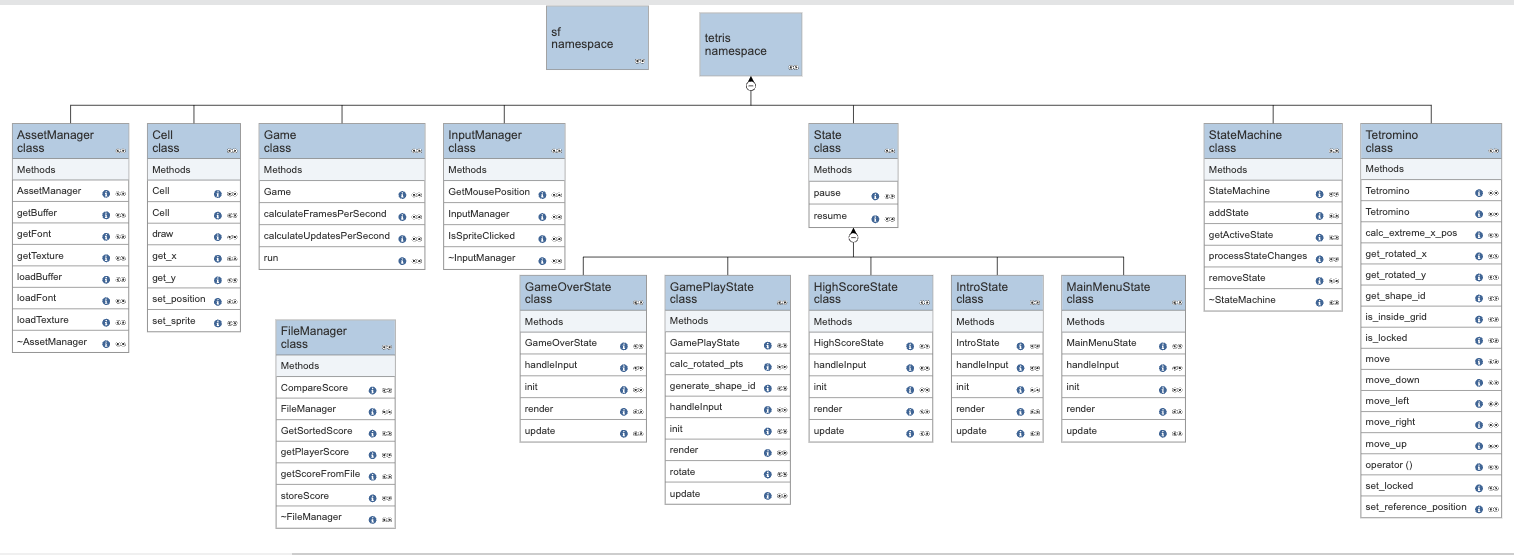
\includegraphics[width=1.2\textwidth]{images/ClassDiagram}
	\caption{Class Diagram of the Game}
\end{figure}


\begin{figure}[H]
	\centering
	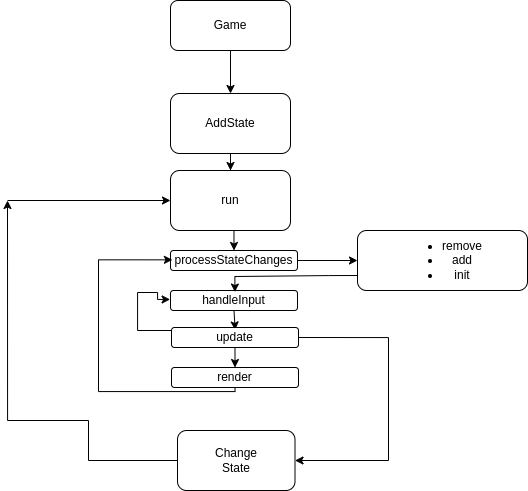
\includegraphics[width=0.7\textwidth]{images/StateMachine.png}
	\caption{Block Diagram: State Machine}
\end{figure}

\begin{figure}[H]
	\centering
	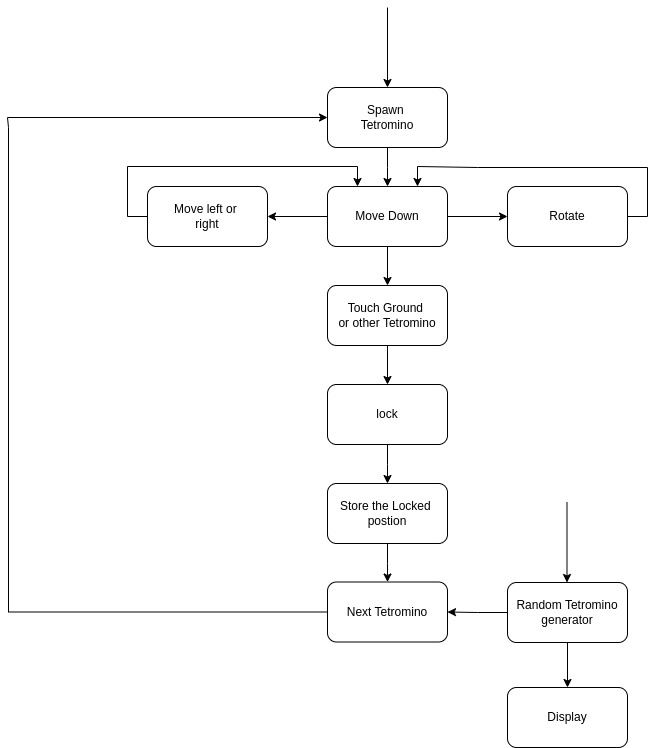
\includegraphics[width=0.7\textwidth]{images/GamePlayBlockDiagram.jpg}
	\caption{Block Diagram: GamePlay}
\end{figure}


  	\newpage
\section{RESULTS}

\hspace{5mm} After the final program was coded, the result obtained was close to what was expected. Game uses keyboard keys for function. Program starts with a short Intropage (for 2 sec) and then Mainmenu loads-up, with Play, HighScore, and Exit buttons. When played, the game goes into play state and game runs.\\ 

When the user gets out, GameOverState loads-up, and he is asked his name for storing his scores in a File. Then he can view top-ten scores in by pressing HighScore button and can press backspace to return back to the mainmenu state.\\
Then  pressing the Exit button will close the gameplay window.\\

\begin{figure}[H]
	\centering
	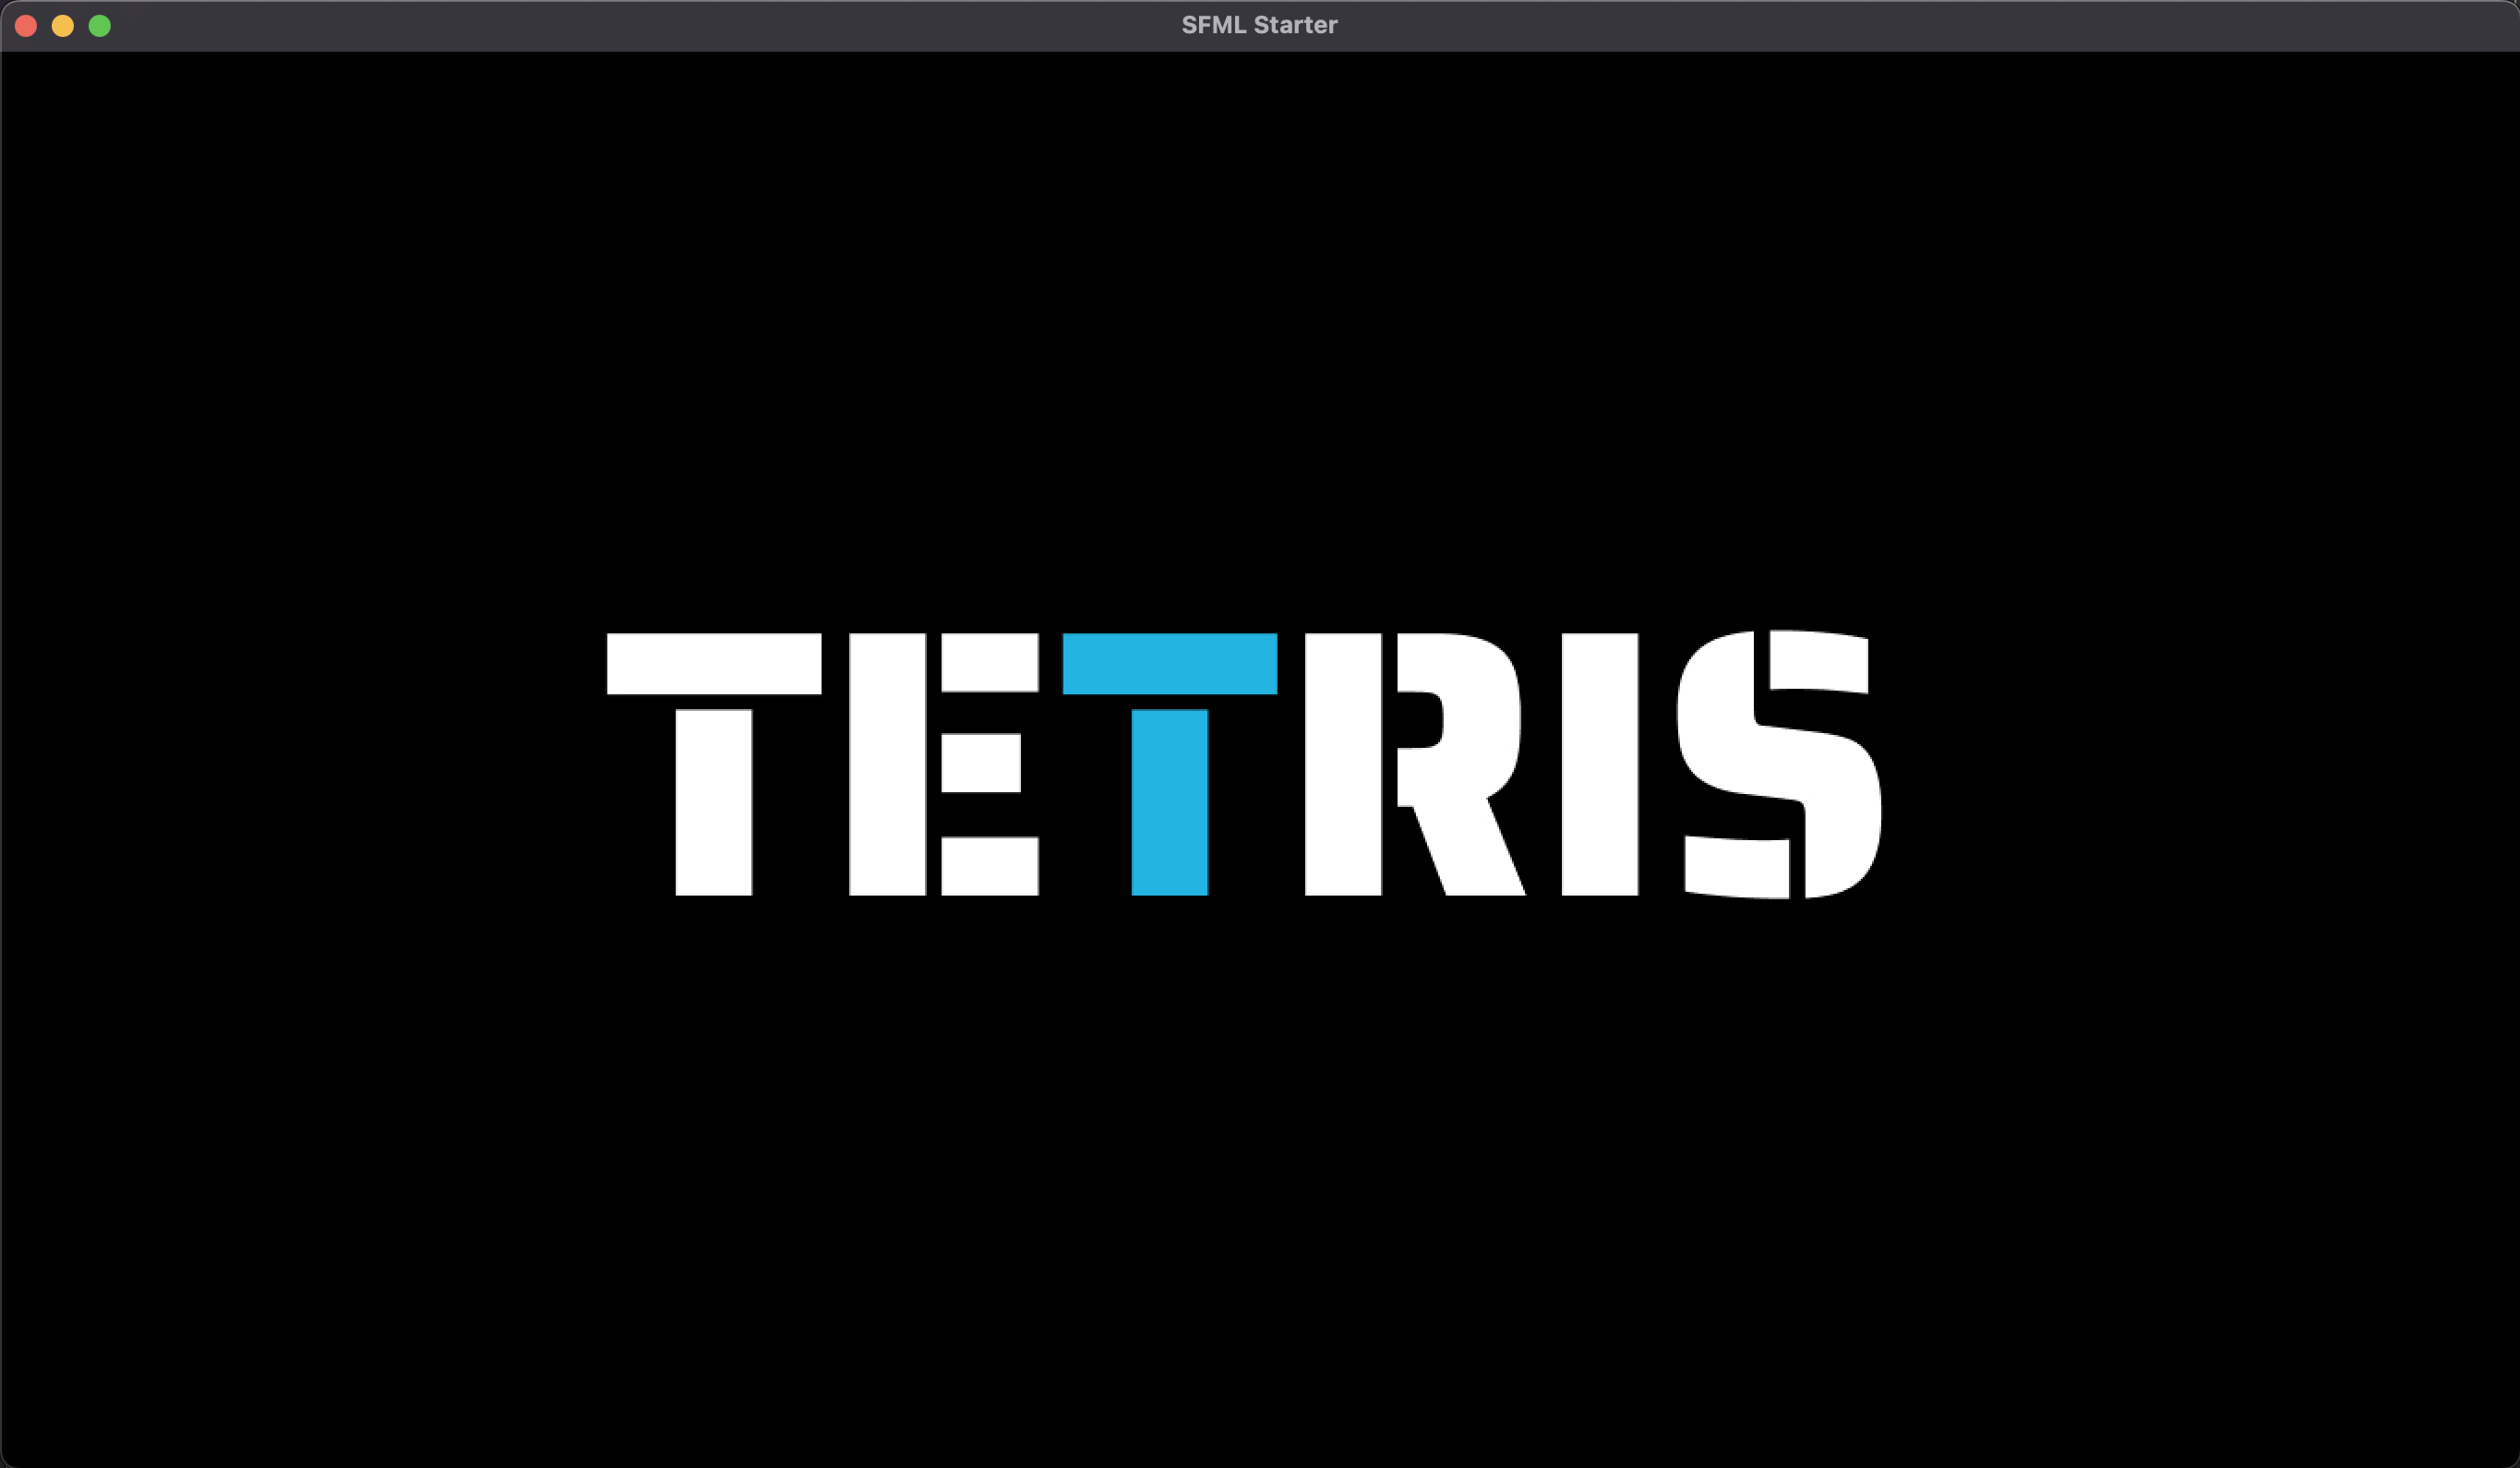
\includegraphics[width=0.9\textwidth]{images/IntroState}
	\caption{IntroState}
\end{figure}

\begin{figure}[H]
	\centering
	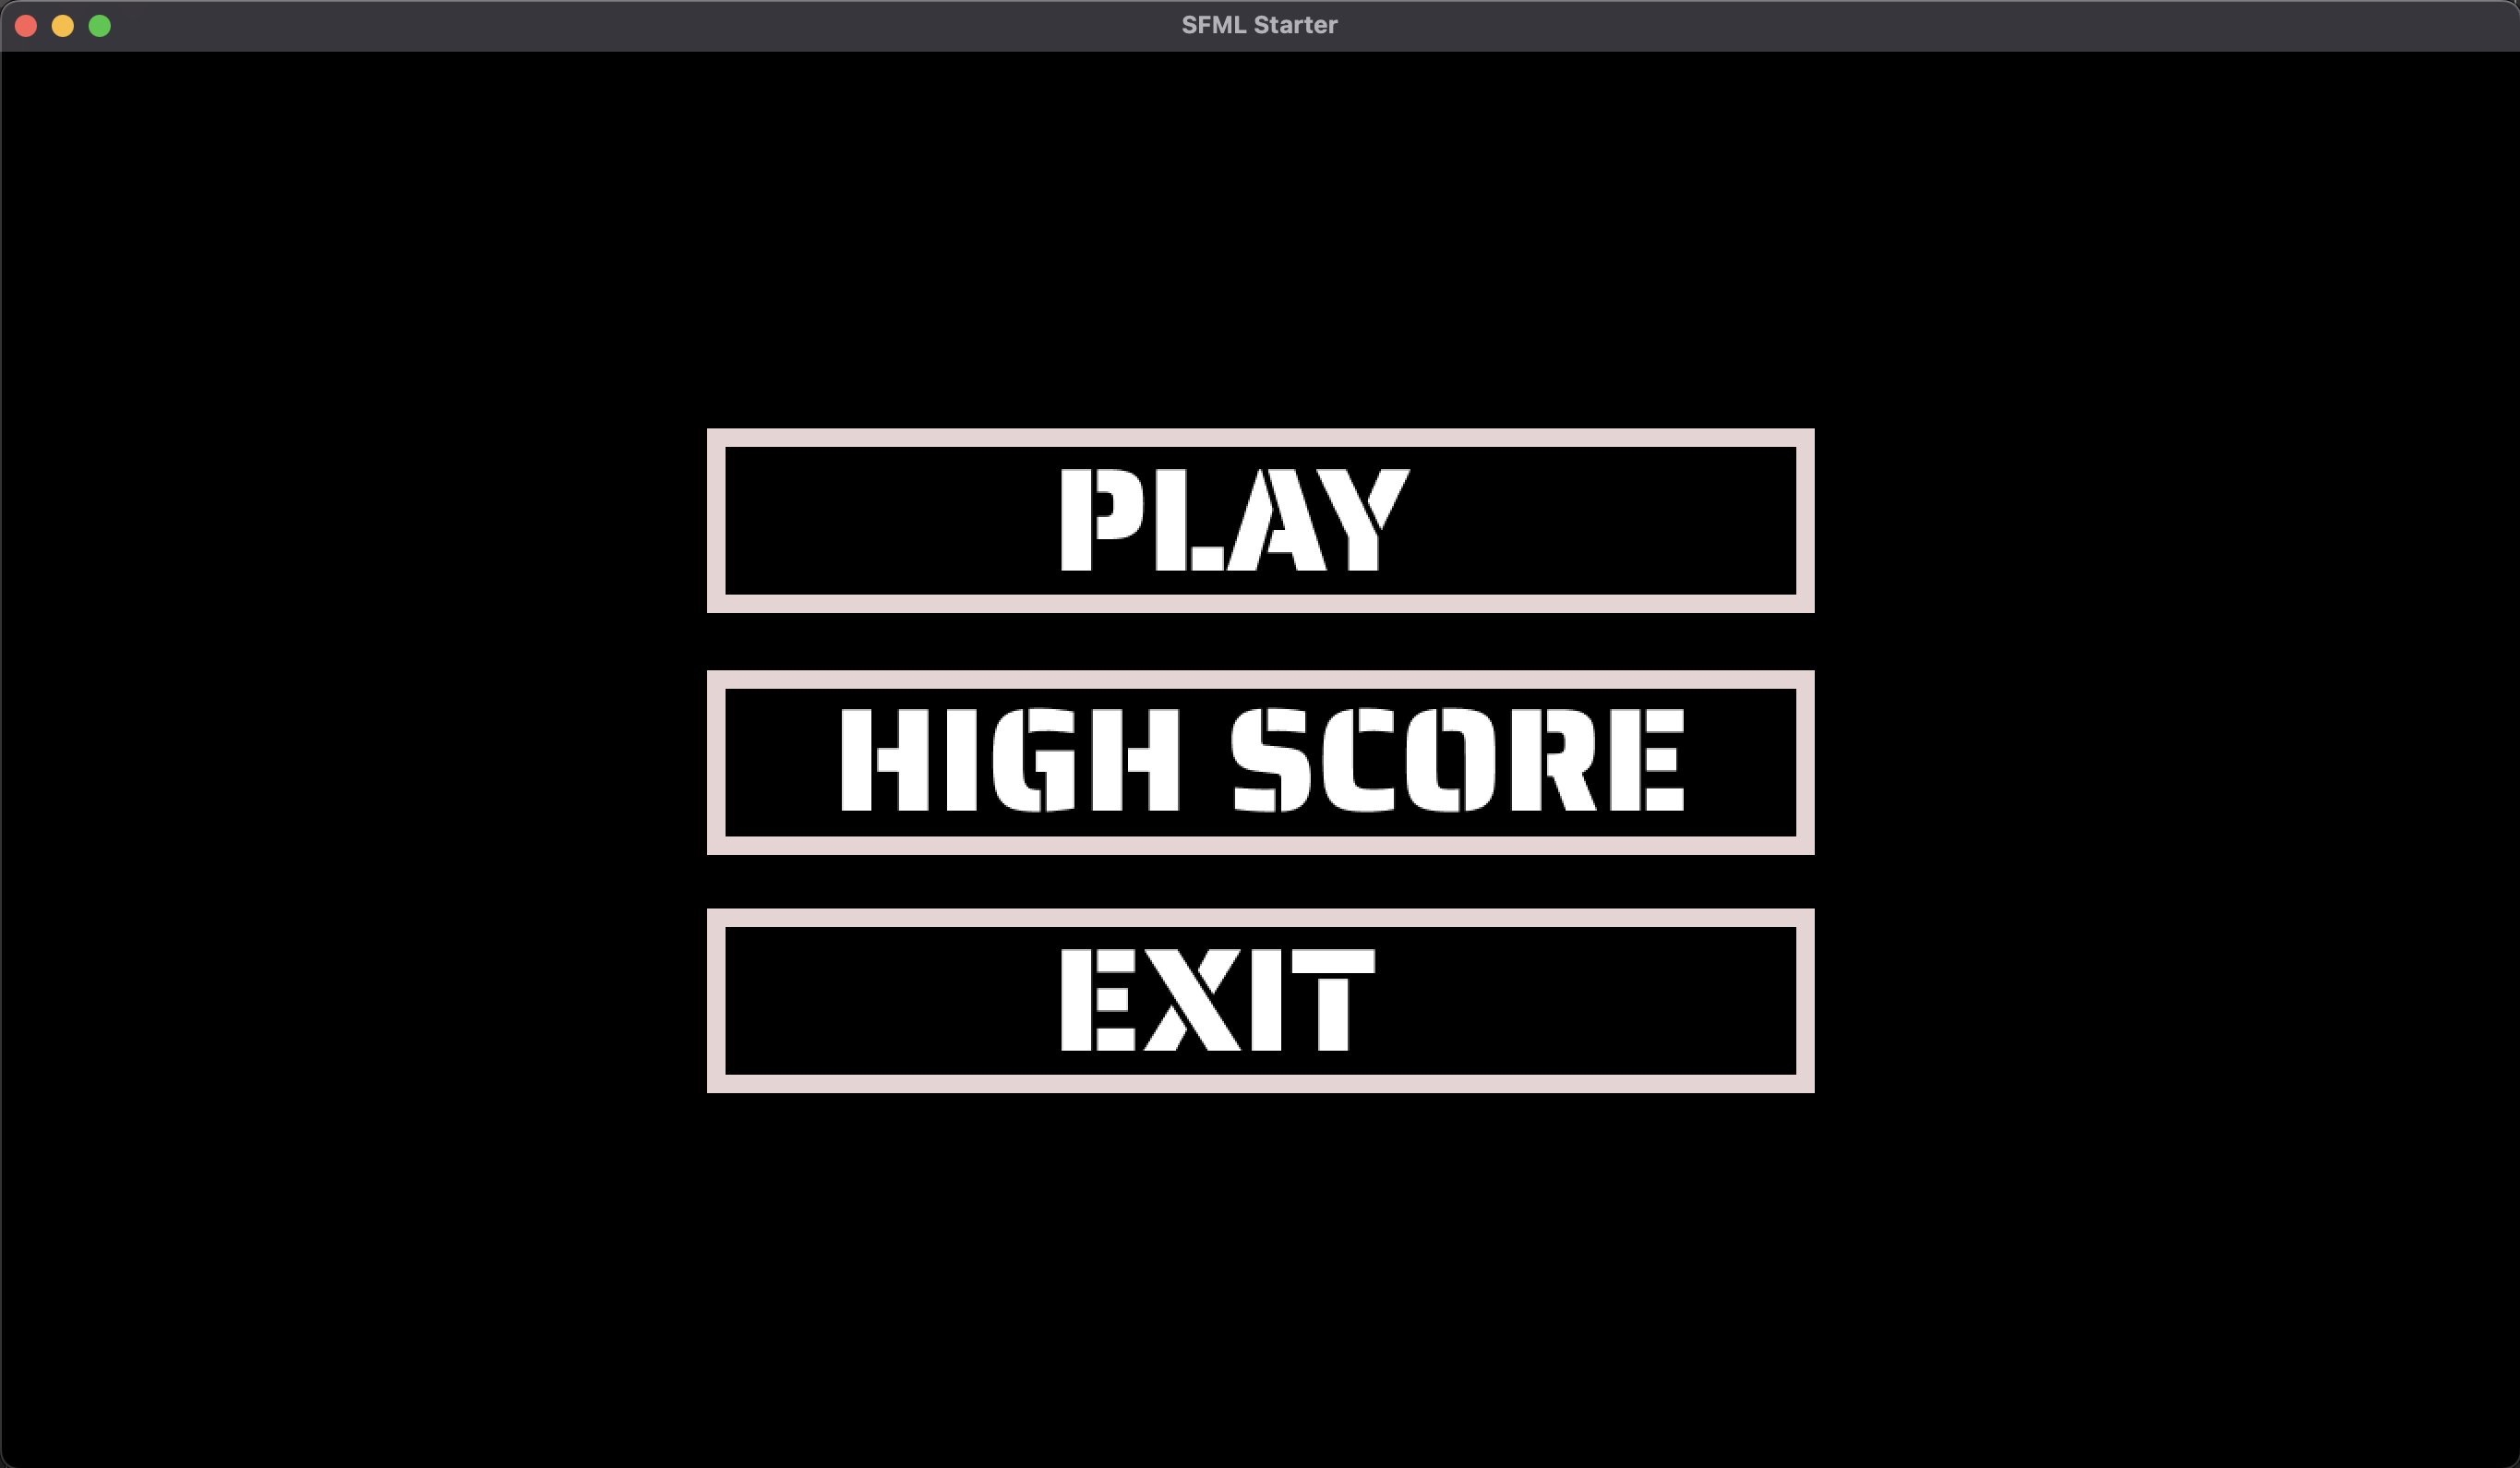
\includegraphics[width=0.9\textwidth]{images/MainMenuState.png}
	\caption{MainMenuState}
\end{figure}

\begin{figure}[H]
	\centering
	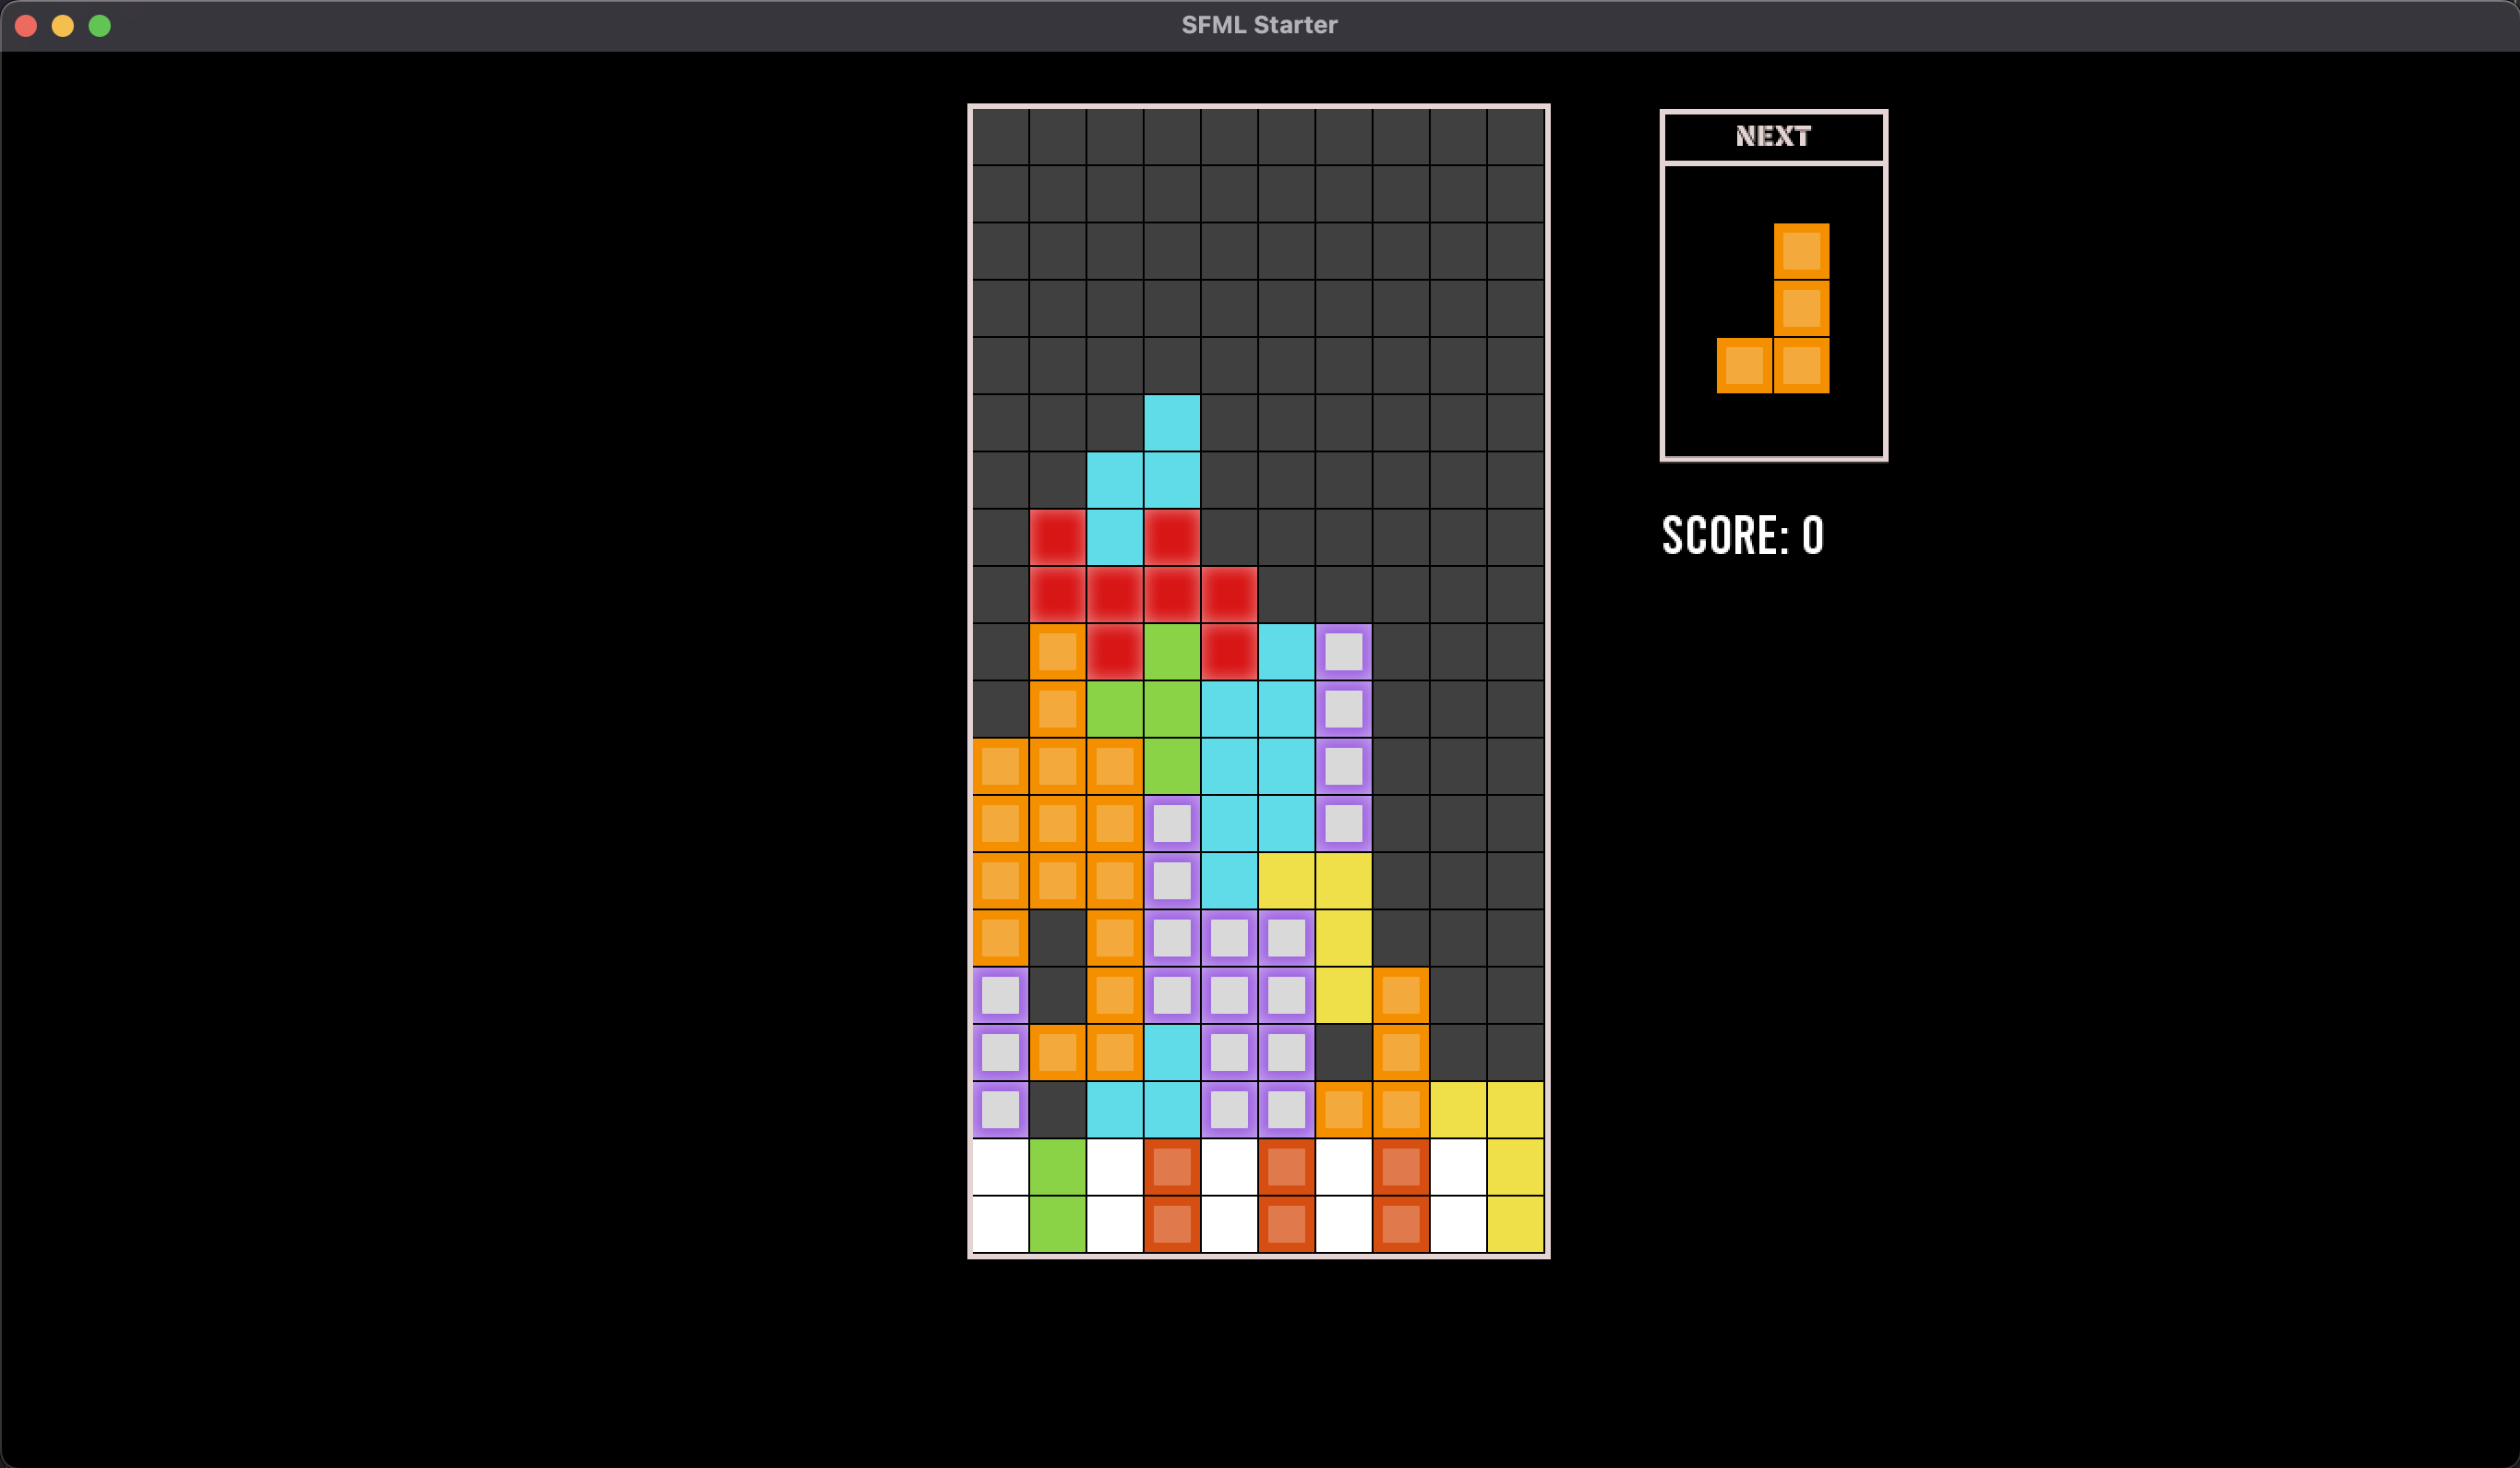
\includegraphics[width=0.8\textwidth]{images/GamePlayState.png}
	\caption{GamePlayState}
\end{figure}
\begin{figure}[H]
	\centering
	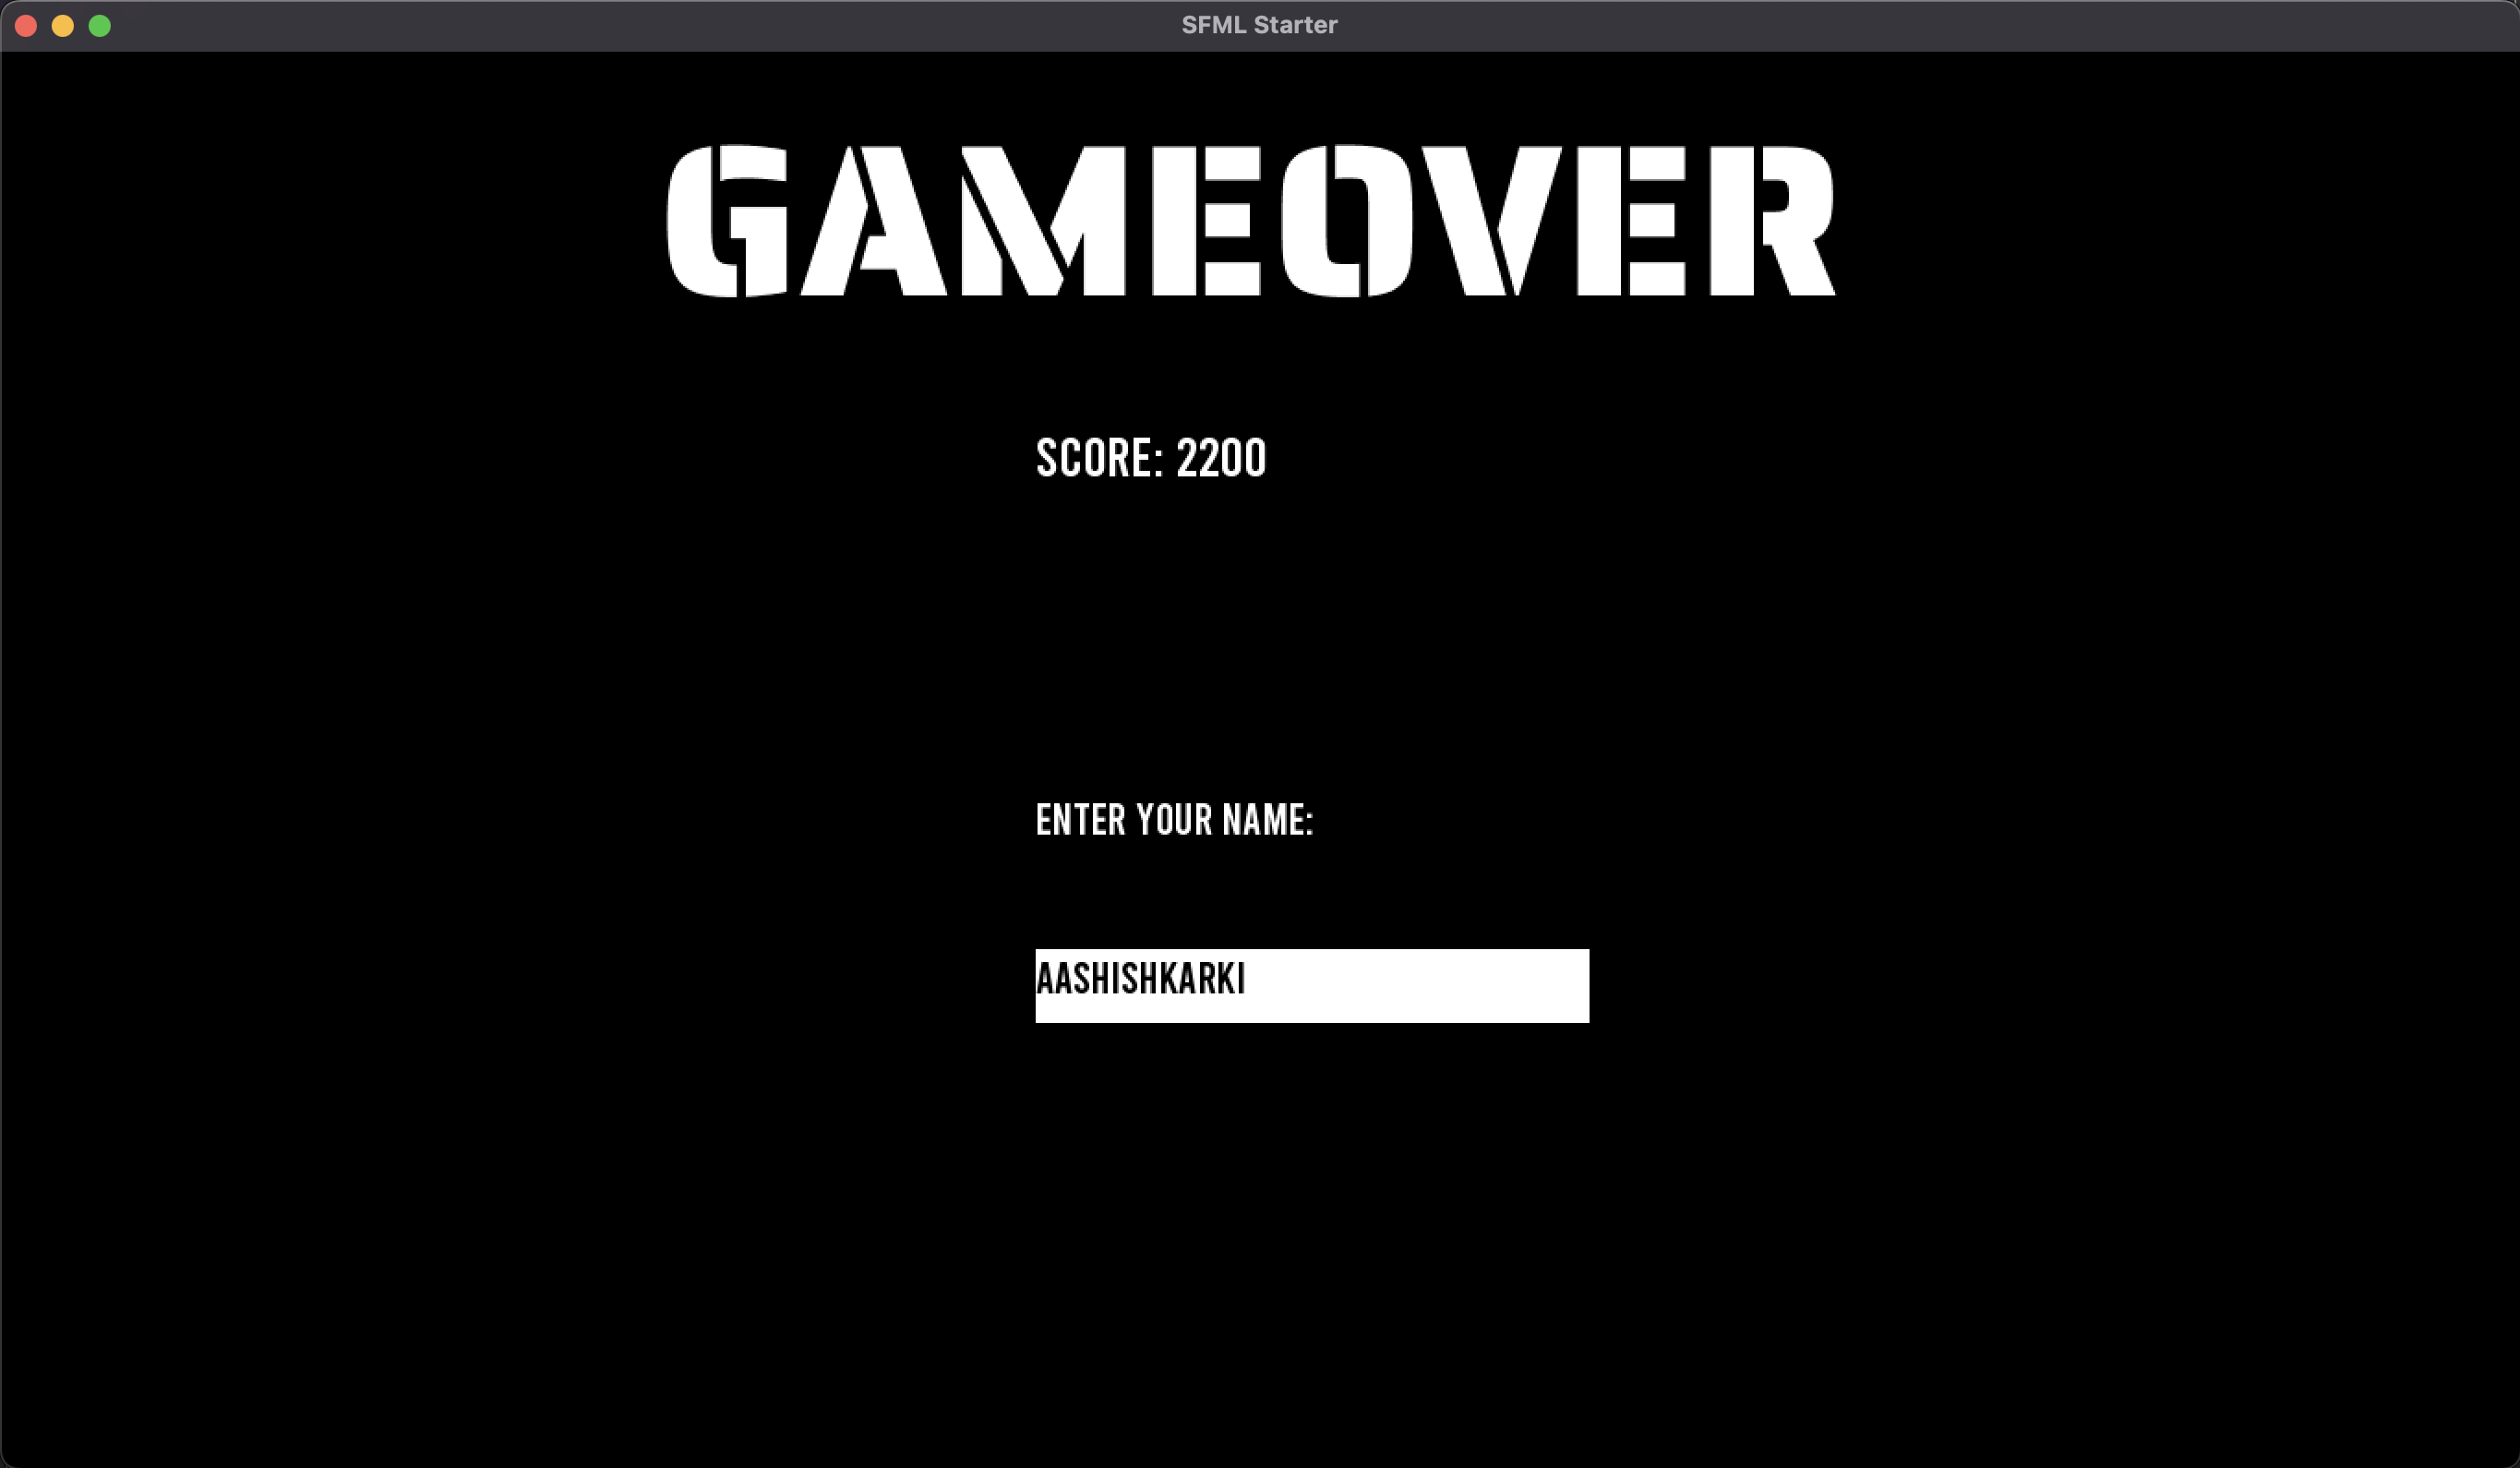
\includegraphics[width=0.8\textwidth]{images/GameOverState.png}
	\caption{GameOverState}
\end{figure}
\begin{figure}[H]
	\centering
	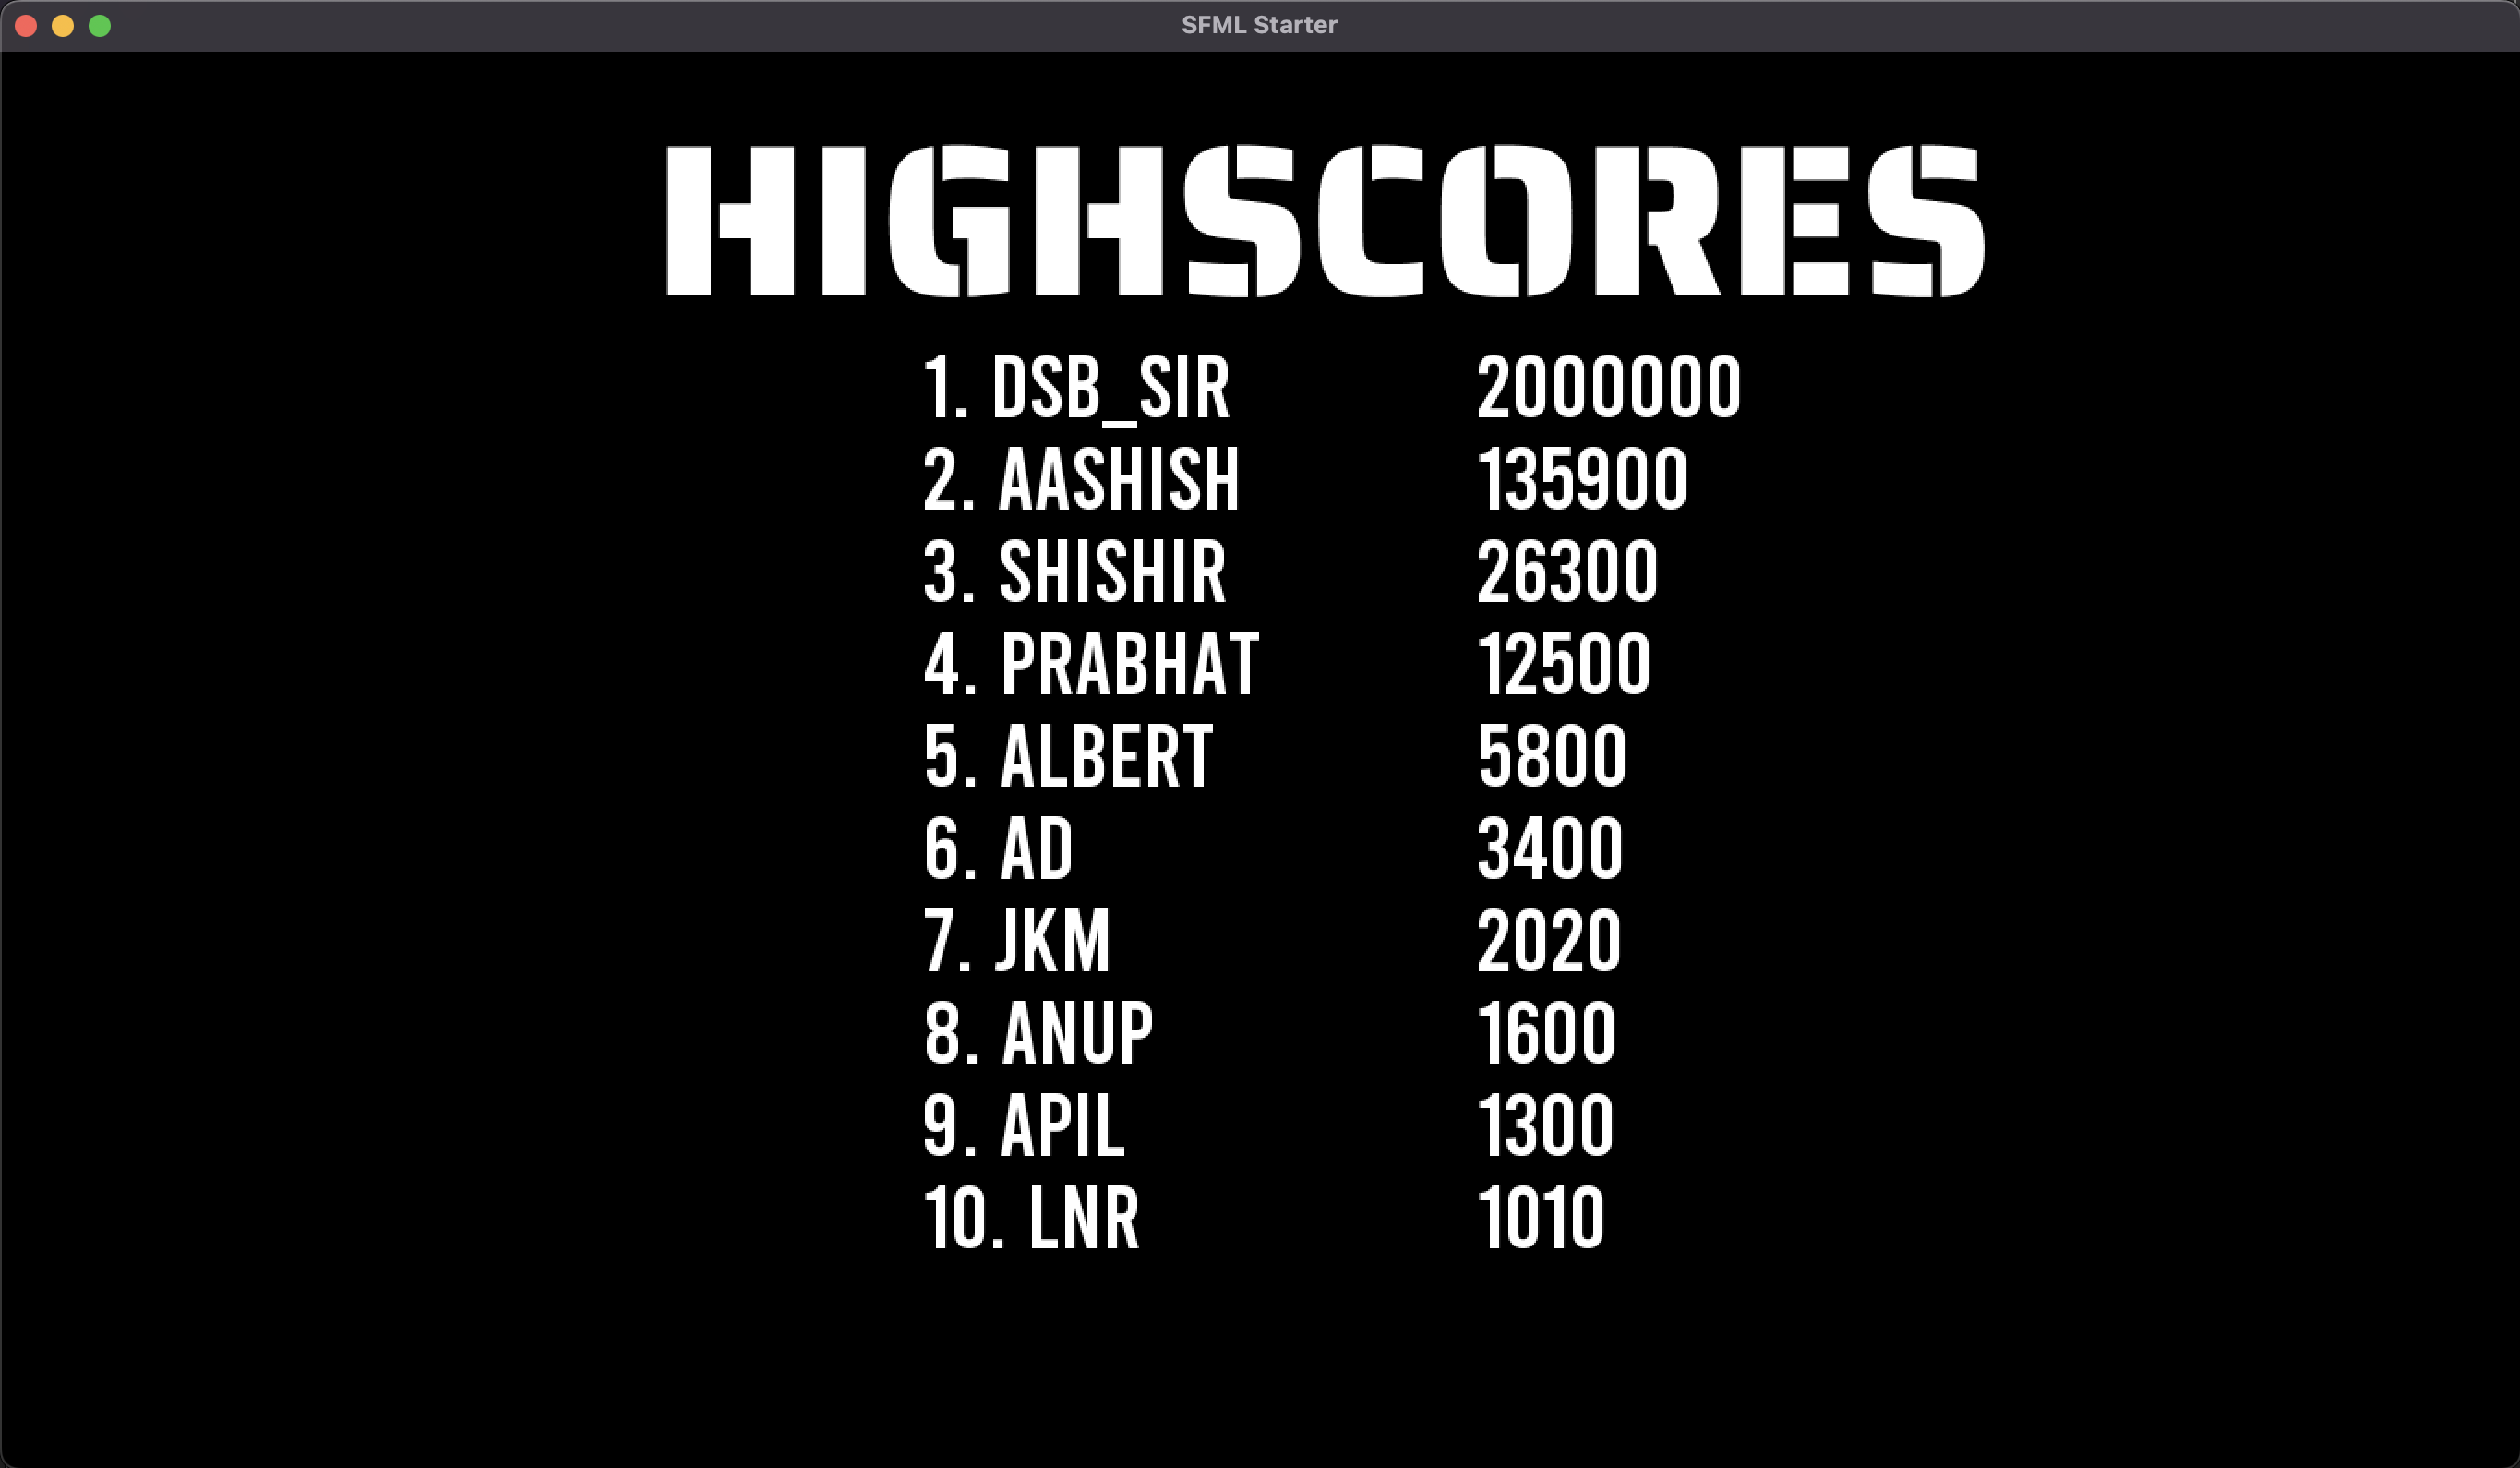
\includegraphics[width=0.8\textwidth]{images/HighScoreState.png}
	\caption{S}
\end{figure}


  	\newpage
\section{PROBLEMS FACED AND SOLUTIONS}
  	\newpage
\section{LIMITATIONS AND FUTURE ENHANCEMENTS}
  	\newpage
\section{CONCLUSION AND RECOMENDATION}
  	\newpage
\section{REFERENCES}

\textbf{Websites :}
\begin{enumerate}

\item https://www.sfml-dev.org/documentation/2.5.1
\item https://github.com/kiswa/SFMLStarter
\item https://geeksforgeeks.com
\item https://stackoverflow.com
\item https://youtube.com

		
\end{enumerate}

\textbf{Books: }
\begin{enumerate}
	\item The Secrets of Object Oriented Programming in C++ -Daya Sagar Baral, Diwakar Baral
	\item Object-Oriented Programming in C++ - Robert Lafore (Fourth Edition)
\end{enumerate}
  	
  	
  	
  	
  	
  
  
  
  
	
\end{document}


